\chapter{Design}
\label{chap:design}
This chapter describes design of the whole platform in details, however implementation specifics of some parts of the tool are described in the following chapter.  This chapter starts with an high-level overview of the complete platform and interactions between the parts and follows by a simple use-case to give the reader idea how this tool is mean to be used. 

Spans and their format are described next followed by design of the native agent and instrumentation server. This chapter ends by describing the used Zipkin user interface and also JSON format in which the user interface accepts the data from the instrumentation server. 

\section{Overview}
\label{design:overview}
Main purpose of this tool is to collect distributed traces. In order to achieve that, the thesis is based on the concept of Spans. Spans are used to denote some specific part of the communication between the communicating nodes and are the important elements for building the whole trace trees. Trace trees consists of several spans and represent the complete task or communication where a span inside the trace represents usually a few remote procedure calls between two neighboring nodes. The node initiating the trace creates so called parent span and new calls started within this span create new nested spans. Created spans can be exported using different span exporters and can be send to the user interface using various data collectors. Span exporters are used to export spans in desired format on disk or on the network for further data collection. The collected data are used for spans visualization in the user interface. The user interface receives the spans from the span exporters or data collectors and present them to the user in a form of trace trees.

Definition of when a new span is to be created and when an existing span needs to be closed is done by a developer by extending the core instrumentation server library. The created instrumentation server is then used for instrumenting the classes of the original application at which information about spans needs to be preserved. In order to obtain the class files, the native agent runs  as part of the monitored application and sends the instrumentation server the desired classes. The native agent is the core part of the whole platform. It is attached to the monitored application and additionally to the instrumentation, it is used to obtain various low-level information from the application. 

The tool therefore consists of three main parts:
\begin{itemize}
	\item Native Agent
	\begin{itemize}
		\item Is used to obtain byte-code for the instrumentation.
		\item Is used to actually apply the instrumented byte-code.
	\end{itemize}
	\item Instrumentation Server
	\begin{itemize}
		\item Instruments the classes obtained from the native agent.
		\item Is also a base library for custom application instrumentation server.
		\item Can contain implementation of custom span exporters.
	\end{itemize}
	\item User Interface
\end{itemize}


The Figure \ref{fig:architecture} denotes the basic relationships between the major parts. Instrumentation server communicates with the native again mainly in order to instrument classes. The application communicates with the user interface by sending the spans to it. The spans can be send either via data collection agent or via one of the default span exporters explained later in this chapter. Each part is explained in more detail later in this chapter. \begin{figure}
	\centering
	
\includegraphics[scale=0.6]{architecture.png}
	\caption{Basic relationship between the major components. }
	\label{fig:architecture}
\end{figure}

The Figure \ref{fig:full_overview} shows how trace trees and spans are related on a simple two nodes example. Each trace is separated from each other trace and represents tracing of a single computation, which consist of several spans. Spans denote more local computation and can also contain additional application-specific information. In order to connect the information from multiple nodes, the trace information needs to be attached to the node communication and that's reason why in this case the methods \texttt{send()}, \texttt{receive()} and \texttt{process()} need to be instrumented. These methods also open and close spans at the correct places in the code.
\begin{figure}
	\centering
	
\includegraphics[scale=0.56]{full_overview.png}
	\caption{Trace and Span demonstration. }
	\label{fig:full_overview}
\end{figure}
\section{Example Use Case}
\label{design:use_case}
In order to demonstrate the use case for which this architecture is a good fit, a simple architecture of a distributed application is shown in this section. The example consists of three modules. The client module used for submitting a task, the execution module and the module used for exporting the data. These modules can be represented as a different threads in a single applications or as separated application nodes. In this example, the user always passes a task to the client module. The client module performs some pre-processing and sends the task to the execution module. This module performs the computation and sends the data to the exporter module, which exports the data on disk and informs the client of the task completion. The architecture of the example can be seen on the Figure \ref{fig:example_arch}.

The goal is to be able to discover how long the transfers between different modules last and how long the processing on each module takes. It is also assumed that the platform does not collect this information already otherwise the cluster monitoring tool would not be required. For simplicity, let's also assume that each module performs the functionality in a single method. The following code sections give the schematic code of each method.

	\begin{figure}
		\centering
		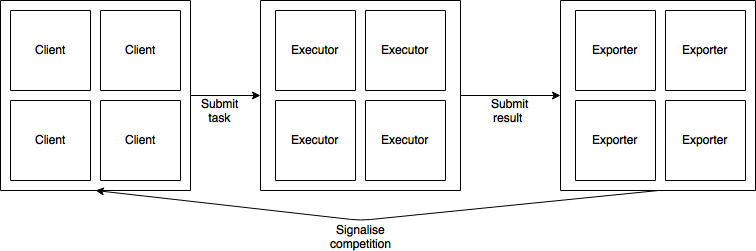
\includegraphics[scale=0.5]{example_arch.png}
		\caption{Example architecture.}
		\label{fig:example_arch}
	\end{figure}



\begin{itemize}
\item \textbf{The client:}
\begin{lstlisting}[language=Java]
public acceptTask(Task task){
  preprocessTask(task)
  ...
  sendTaskForComputation(task)
  ...
  waitForExporterToFinish()
  ...
}
\end{lstlisting}

\item \textbf{The executor:}
\begin{lstlisting}[language=Java]
public execute(Task task){
  TaskResult result = executeTask(task)
  ...
  sendResultForVisuzalization(result)
}
\end{lstlisting}

\item \textbf{The exporter:}
\begin{lstlisting}[language=Java]
public export(TaskResult result){
  saveToDatabase(result)
  ...
  notifyClient()
}
\end{lstlisting}
\end{itemize}

In order to be able to collect this type of information and be able to reason about the relationship between the nodes, these methods needs to be instrumented. The instrumented code should look as in the schematic code bellow. For achieving this, the developer is supposed to extend the instrumentation server which acts as the base library and provides the developer with several helper methods used to specify the instrumentation points for their applications. 

\begin{itemize}
\item \textbf{The instrumented client:}
\begin{lstlisting}[language=Java]
public acceptTask(Task task){
  TraceContext tc = TraceContext.create()
  tc.attachOnObject(task)
  Span s = tc.openSpan("Main Client Span")	
  s.addAnnotation("tskReceived", timestamp)
  ...
  preprocessTask(task)
  s.addAnnotation("tskPreprocessed", timestamp)
  ...
  sendTaskForComputation(task)
  ...
  Result res = waitForExporterToFinish() // blocking method
  ...
  tc.closeCurrentSpan()
}
\end{lstlisting}
The \texttt{create} method creates a new trace and the \texttt{attachOnObject} method attaches the trace context on the \texttt{task} object, which is passed around the network. The method \texttt{openSpan} opens a new span encapsulating the client computation. The \texttt{addAnnotation} method is used to add application specific information to the current span. The \texttt{closeCurrentSpan} method is used to close the current span and export the content using the provided span exporter. In the default case, the data are sent to the user interface directly.


\item \textbf{The instrumented executor:}
\begin{lstlisting}[language=Java]
public execute(Task task){
  TraceContext tc = TraceContext.getFromObject(task)
  tc.openSpan("Executor span")
  TaskResult result = executeTask(task)
  tc.attachOnObject(result)
  ...
  sendResultForExport(result) // non-blocking method
  tc.closeCurrentSpan()
}
\end{lstlisting}
In this case, we don't create a new trace context but get the existing one from the \texttt{task} object on the input. A new nested span is created. This span has the original span created within the client application as its parent.

\item \textbf{The instrumented exporter:}
\begin{lstlisting}[language=Java]
public export(TaskResult result){
  TraceContext tc = TraceContext.getFromObject(result)
  tc.openSpan("Exporter span")
  saveToDatabase(result)
  ...
  tc.closeCurrentSpan()
  notifyClient()	
}
\end{lstlisting}
In this case, the meaning of the methods is the same as above.

\end{itemize}

The developer should extend the base instrumentation server by steps how to instrument the classes  in order to have a similar format as above. The extended instrumentation server is described on the Figure \ref{fig:example_extended}.

	\begin{figure}
		\centering
		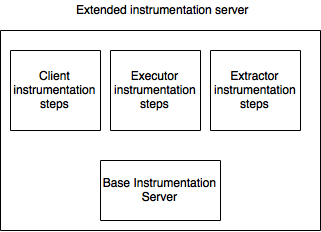
\includegraphics[scale=0.5]{example_extended.png}
		\caption{Structure of extended instrumentation server JAR.}
		\label{fig:example_extended}
	\end{figure}

The extended instrumentation server is then run on each node or on the network and is used to perform the instrumentation requested from the application. The native agent has to be attached to all nodes of distributed application prior it's start and the path to the extended instrumentation server JAR needs to be set as an mandatory argument. The default span sever is used in this case and the collected spans are send right to the Zipkin UI. The default endpoint for the user interface is used when not defined as an argument to the native agent. 

A single collected trace from this application should look as shown on the Figure \ref{fig:example_trace}.

	\begin{figure}
		\centering
		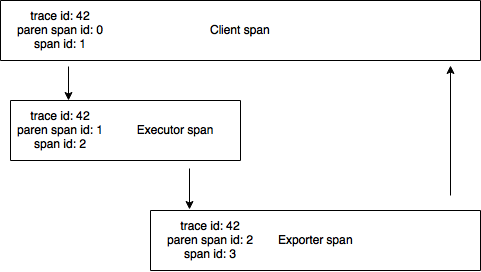
\includegraphics[scale=0.5]{example_trace.png}
		\caption{Example trace in case of the example application.}
		\label{fig:example_trace}
	\end{figure}

Therefore, it can be seen that the only part the developer needs to work with is the extension of the instrumentation server to specify the custom instrumentation points, otherwise the rest of the work is done automatically. The end user is only responsible for starting the application with the agent attached.

\section{Spans and Trace Trees}
\label{subsec:spans}
As mentioned briefly in the previous section, spans are used to gather the information about the distributed calls or so called, distributed stack traces. Points in the code where spans are created and closed are defined as part of the Instrumentation server but since it's the most important concept in the thesis, we explain them in the separated section. 

Spans are the main concept behind capturing the distributed traces. They are special classes which instances are injected to instrumented application's classes to keep track of the communication and the state between the nodes in the distributed application. Usually, the initiator creates so called parent span and new calls started within the span create new nested spans. Collected spans can be processed using different span exporters and can be sent to the user interface using various data collectors.

Spans has several mandatory and optional fields. The mandatory fields are trace id, span id and parent span id. Trace id identifies one complete distributed call among all interacting nodes on the cluster. This field is attached automatically when a new root span is created. Root span is a first span created inside a trace. The root span does not have parent id field set up and therefore the user interface back-end can distinguish between regular spans and root spans and therefore can identify the start of the whole trace. Parent id of a span is always id of span from which the span received a request to perform some task. The span and its parent span can be located on the same node or on different nodes as well. The first variant can be useful in cases where the developer requires to trace several threads as separated spans within a single node.  

Span have several additional fields, which are later used in the user interface. The fields are:
\begin{itemize}
	\item \textbf{Timestamp} - when the span started.
	\item \textbf{Duration} - how long the span lasted.
	\item \textbf{Annotations} - annotations which are used to carry additional timing information about spans. For example time when span has been received on the receiver side or the time the span has been processed at the receiver side can be set using the annotations.
	\item \textbf{Binary annotations} - annotations which can be used to carry around application specific details. We can use these annotations to transfer information between communication nodes inside of spans. For example, one node can store number of bytes sent during the request and the receiver can use this information to calculate overall number of bytes received from this particular node.
\end{itemize}
Each span has also an internal field called \textbf{flags}. The developer may store flags important to the instrumentation and these flags are transferred as part of the spans. Flags are not sent to the user interface and are only used for instrumentation purposes.

Each annotation, both binary and regular, has also endpoint information attached. This element consist of:
\begin{itemize}
	\item \textbf{IP} - IP of the node on which this event was recorded
	\item \textbf{port} - port on which the service which recorded the span is running.
	\item \textbf{service name} - service name which is used to group different traces by names and can be later used to filter traces using this field in the user interface.
\end{itemize}

\subsection{Span IDs}
It is also important to mention that span id and parent span id are created randomly. This is done in order to allow parallel spans in the same control flow without overlapping as can be seen on the Figure \ref{fig:parallel_spans}.

	\begin{figure}
		\centering
		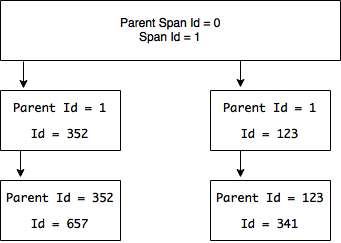
\includegraphics[scale=0.6]{parallel_spans.png}
		\caption{Generating span ids randomly ensures that they don't overlap when they are created in parallel.}
		\label{fig:parallel_spans}
	\end{figure}
If the ids were not random at different nodes of the distributed system, the parallel spans would be creating child spans with ids in the same linear sequence and therefore these spans would be overlapping, as can be seen on the Figure \ref{fig:parallel_spans_overlapping}
	\begin{figure}
		\centering
		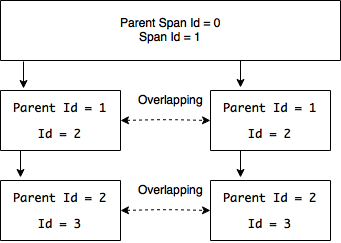
\includegraphics[scale=0.6]{parallel_spans_overlapping.png}
		\caption{Generating span with the same linear sequence leads to span overlapping.}
		\label{fig:parallel_spans_overlapping}
	\end{figure}
	
The following sections contain information about how spans are exported for external communication with the user interface and also how spans are created using \texttt{TraceContext} and \texttt{TraceContextManager} classes.
\subsection{Span Exporters \& Data Collectors}
Spans are exported from the application using the span exporters. Span exporter for the application may be selected via one of the native agent configuration properties. It is important to mention that all spans in the application are using the same, because span exporter is static field of the \texttt{Span} class. Span exporters need to be available to the monitored application and therefore are brought to the application from the instrumentation server via the native agent during the agent initialization phase.

The Distrace tool includes two default implementation of span exporters, but also allows the developer to create new span exporters. Custom span exporters may be useful in cases when the developer wants to export the span data in a format used by different user interface or to use custom data collector. Data collector is a service which collects the data from the specified place and store them in central data storage available by all application's node. This thesis does not implement data collection service as many services exists for this purpose. 

Data collected within spans are internally represented in JSON format understandable by the Zipkin user interface. This is also the reason why the thesis contains support for working with JSON data and it is explained in more detail later in the Chapter \ref{chap:implementation}. This format can be again changed by the custom span exporter.

Span exporter implementations need to extend from the abstract ancestor defining common methods for each span exporter. Also, in order to be able to use the exporter automatically in the code, it has to have a constructor with single \texttt{String} argument accepting exporter arguments. The arguments format is defined in the case of default span exporter, however the developer may use any format in case of custom span exporters. The common ancestor, \texttt{SpanExporter} abstract class has two abstract methods:
\begin{itemize}
	\item \texttt{export}. This method is used for exporting the span. Custom span exporter implementation may save the data on local disk or send over network. The destination is not limited by the code. Internally, the \texttt{saveSpan} method is called asynchronously in a separated thread to allow asynchronous span processing, which has a performance benefit.
	\item \texttt{parseAndSetArgs}. The instrumentation agent accepts also special argument which contains arguments for the defined span exporter. Each span exporter is responsible for parsing the span exporter arguments.
\end{itemize}

As mentioned above, the tool provides two default simple span exporters:
\begin{itemize}
	\item  \texttt{DirectZipkinExporter} - The default span exporter sends the collected span asynchronously to the user interface right away without storing the data on disk to be collected by an external data collector. In this case the functionality of the span exporter and the data collector are handled by this single . This span exporter should be used for demonstration purposes only since it could overload the user interface or network when processing and sending high amount of collected spans in a short amount of time to the user interface as the UI is not prepared to store large amounts of data in the memory. 
	
	This exporter accepts a single argument, which is IP and port of the Zipkin UI service. The Figure \ref{fig:zipkin_span_exporter} shows how the Zipkin span exporter is used.
	
		\begin{figure}
			\centering
			
\includegraphics[scale=0.6]{zipkin_span_exporter.png}
			\caption{Using the Zipkin span exporter to export spans directly to Zipkin user interface without the data collector agent.}
			\label{fig:zipkin_span_exporter}
		\end{figure}
	\item  \texttt{JSONDiskExporter} - The second available span exporter saves the collected data asynchronously on disk in the format known to Zipkin UI for future collection to the Zipkin user interface by custom data collector. Together with some well-known data collection agent, this is a preferred way of transferring spans from the application to the Zipkin user interface in the production. This exporter accepts single argument which is a directory where collected spans are saved. The Figure \ref{fig:disk_span_exporter} shows how JSON disk span exporter is used.
	\begin{figure}
		\centering
		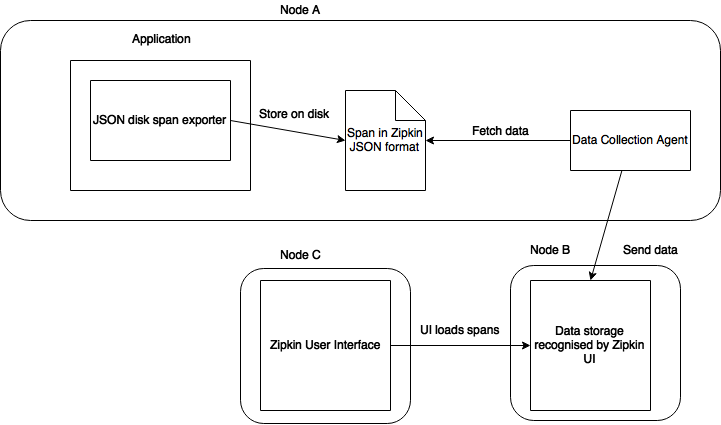
\includegraphics[scale=0.5]{disk_span_exporter.png}
		\caption{Using the JSON disk exporter together with the data collection service but Zipkin user interface .}
		\label{fig:disk_span_exporter}
	\end{figure}
\end{itemize}
Additionally, the Figure \ref{fig:custom_span_exporter} shows how a custom span exporter may be used.

\begin{figure}
	\centering
	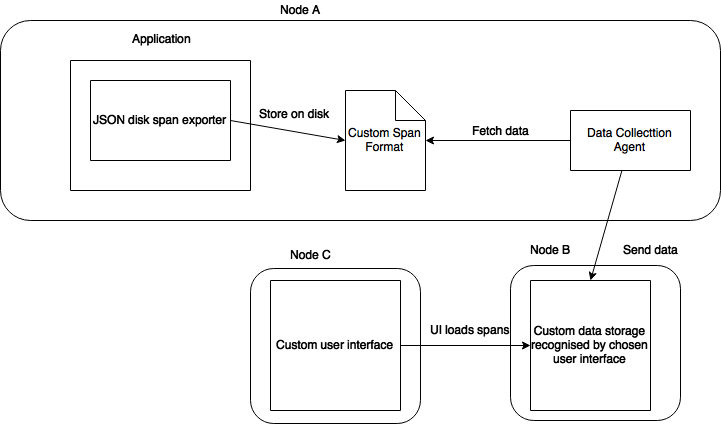
\includegraphics[scale=0.5]{custom_span_exporter.png}
	\caption{Using custom span exporter together with the data collection service and custom user interface.}
	\label{fig:custom_span_exporter}
\end{figure}
In order to give the developer the flexibility to add new exporters without changing the internals, the span exporters have to be  registered in the META-INF directory of the extended instrumentation server JAR file. This ensures that the service loader can find all implementations of the \texttt{SpanExporter} abstract class. The reason why the classes need to be discovered is explained in the following Section \ref{native_agent_design}

To make the developer life easier, the \textbf{AutoService} library\footnote{The AutoService library is available at \url{https://github.com/google}.} is used. Instead of manually registering the implemented span exporters into META-INF directory, they can be annotated in the code using the \texttt{AutoService} annotation with a single argument specifying the abstract parent, in this case \texttt{SpanExporter}. The library takes care of registering the classes automatically in the desired folder in correct format so the human error is minimized.

\subsection{Trace Context}
Trace context is a class used for storing the information about the current span and also for creating new spans and closing current spans. Trace context is always attached to a specific thread. This is done in order to allow multiple threads to have different computation state and therefore the platform is able to capture multiple distributed traces at the same time on the same node. Singleton instance of class \texttt{TraceContextManager} is used for attaching the threads to the trace contexts and vice-versa. It has a few methods allowing the developer to attach trace context to a specific thread and also to get trace context which is attached to a current thread.

Each trace is represented by trace context and is uniquely identified by Universally unique identifier (UUID) of type one\footnote{More UUID versions exist and are created based on different information}. This UUID type combines 48-bit MAC address of the current device with the current timestamp. This way it is ensured that two traces created at the same time on different nodes can't have the same identifier. The identifiers are created in the native agent using C++ library called Sole\footnote{The Sole library is available at \url{https://github.com/r-lyeh/sole} and can be used to create identifiers in C++ language.} and are made available to the Java code via a published native method \texttt{getTypeOneUUID}.

The trace contact has methods \texttt{openNestedSpan} and \texttt{closeCurrentSpan}. The first method is used to create a new nested span and set the newly created span as the current one. Nested span is a span which sets its parent id to the current span. A root span is created in case when no current span exists. The second method is used to close the current span. Closing the span triggers the span exporting operation using the configured span exporter and the parent span becomes the current span.

The Figure \ref{fig:closing_spans} shows how spans are created, closed and saved.  in this chapter. \begin{figure}
	\centering
	
\includegraphics[scale=0.6]{closing_spans.png}
	\caption{Creating and closing spans.}
	\label{fig:closing_spans}
\end{figure}

\subsection{Transferring Span Information}
In order to capture the shared state between the nodes in the application or even between the threads on the same application node, the span details and trace context have to be transferred between the threads or between the nodes. Distrace prepares several methods for attaching trace context to either current thread or an object which acts as an carrier of the span information.

Usually when transferring the trace context between the threads on the same node the copies of the trace context have to be used. When transferring the trace context between the different nodes this is not an issue.

The methods the developer can use for obtaining and attaching the trace context are:
\begin{itemize}
	\item \texttt{static create()} - creates a new trace context.
	\item \texttt{static getFromObject(holder)} - gets the existing trace context from the holder object.
	\item \texttt{static getFromThread(thread)} - gets the existing trace context from the specified thread.
	\item \texttt{static getFromCurrentThread()} -  gets the existing trace context from the current thread.
	\item \texttt{attachOnObject(holder)} - attaches the trace context to the holder object.
	\item \texttt{attachOnThread(thread)} - attaches the trace context to the specified \newline thread.
	\item \texttt{attachOnCurrentThread()} - attaches the trace context to the current \newline thread.
	\item \texttt{deepCopy} - creates a deep copy of the trace context. It is usually used in cases where child spans are processes in parallel by multiple threads. In this case, the copy of trace context with the same id is shared among all these threads, but they operate on very own object. This is done in order to be able to monitor parallel spans within a single trace without having to face race conditions on a single trace context object.
\end{itemize}
The methods above can also be chained and for example a trace context can be obtained from the holder object, deep copy created and the newly created copy attached to a new holder object.

There are also different variants how spans can be closed. Span can either closed by the same node or thread who created it. In this case attaching the trace context information to the current thread is usually sufficient. It is also however possible that span can be closed by different thread or node then where it was initially created. In this case the copy of a trace context is usually created and attached to an object which acts as an carrier of the trace information.
\section{Native Agent}
\label{native_agent_design}
The native agent is used for accessing the internal state of the monitored application and also to instrument classes so they can carry the span and trace identifiers between the application nodes. The main agent task is to check whether a class is required to be instrumented and if yes, send the class for the instrumentation to the instrumentation server and wait for the instrumented code.

The native agent consist of several parts. The most important parts are:
\begin{itemize}
	\item \textbf{Bytecode parsing module}. \newline The classes in this module are used to parse the JVM bytecode in order to discover the classes dependencies for further instrumentation. Byte code parsing is a technical task described in the Chapter \ref{chap:implementation}.
	\item \textbf{InstrumentorAPI}. \newline The \texttt{InstrumentorAPI} class provides several methods which are used to communicate with the instrumentation server JVM. All the queries to the server are done via instance of this class.
	\item \textbf{AgentCallbacks}. \newline All callbacks used in the native agent are defined in this namespace.
	\item \textbf{AgentArgs}.  \newline The \texttt{AgentArgs} class contains all the logic required for argument parsing.
	\item \textbf{NativeMethodsHelper}. \newline The \texttt{NativeMethodsHelper} class is used for registering native methods defined in C++. These methods can be later used from the Java code without worrying of the low-level implementation.
	\item \textbf{Utilities module}. \newline This module contain several utility namespaces. The most important utility namespaces are \texttt{AgentUtils} and \texttt{JavaUtils}. The first one contains methods for managing the JVMTI connection and for registering the JVMTI callbacks and events. The second one is used to simplify work with Java objects in the native code via JNI. 
\end{itemize}

\subsection{Agent Initialization}
The agent is initialized through the same phases as described in the Section \ref{subsec:jvmti_init}. The following JVMTI events are especially important to the thesis: \texttt{VM Init}, \texttt{VM Start}, \texttt{VM Death}, \texttt{Class File load Hook}, \texttt{Class Prepare} and \texttt{Class Load}. Callbacks are registered for all the mentioned events so the native agent can react to them accordingly in the code.

As part of the initialization process, the agent is responsible for either connecting to or starting a new instrumentation server. In case the native agent was started in the shared mode of the instrumentation server, the agent tries to connect to already existing server and the server is shared between all application's nodes. In the local instrumentation mode, the instrumentation server is started as a separated process automatically and the connection is established with the server using the inter process communication. In this case, each application node has dedicated instrumentation server.

The callback registered for the \texttt{VM Init} event is responsible for loading all additional classes from the instrumentation server as part of the initialization as well. The additional classes are for example \texttt{Span}, \texttt{TraceContext} or custom implementations of \texttt{SpanExporter} abstract class. These classes are used in the instrumented code and therefore have to be available to the monitored application. The native agent is designed in a way that developers are not supposed to change the code of if. All the extension are supposed to be done within the instrumentation server. Therefore, the instrumentation server is asked at the initialization phase for the list of all additional classes and they are sent to the native agent. The agent puts all the received classes on the application's class-path so they are available to the instrumented code.

\subsection{Instrumentation}
Code for handling the instrumentation is part of the callback for the \texttt{Class File load Hook} event. The callback has the bytecode for the class being loaded as its input parameter and allow the developer to pass a new instrumented bytecode as the output parameter. The process of instrumentation is described here, however the technical details are described in the following chapter.

The process consist of several stages:
\begin{enumerate}
	
	\item Enter the critical section. It can happen that the class file load hook is triggered multiple times and in order to not confuse the instrumentation server, the lock has to be acquired before the instrumentation of a class starts.
	\item Firstly, the check whether the virtual machine is started is done. If the virtual machine is started and initialized, the instrumentation continues, otherwise the instrumentation for currently loaded class is skipped without asking the instrumentation server since it the class is a system class and it is not desired to instrument Java system classes at this moment.
	\item Attach JNI environment to the current thread. Since the JVMTI and JNI does not have automatic thread management, it's up to the developer to take care of correct threading management.
	\item Discover the class-loader used for loading the class
	\item Parse the name of the class being loaded. Even though the callback provides input parameter which should contain the name of loaded class, at some circumstances it can be set to \texttt{NULL} even though the class name is available in the bytecode. Instead of relying on this parameter, the bytecode is parsed and the class name is found manually.
	\item Decide whether the instrumentation should continue. This check is based on the used class loader and name of the class being loaded. Classes loaded by the \texttt{Bootstrap} class loader and in case of Oracle JVM, classes loaded by \texttt{sun.reflect.DelegatingClassloader} are not supposed to be instrumented. 
	The \texttt{Bootstrap} class loader is used to load system class and the second mentioned class loader is used to load synthetic classes and in both cases, it's not desired to instrument classes loaded by these class loaders.
	There are also some ignored classes for which the instrumentation is not desired. Example of these classes are the classes loaded during initialization phase from the instrumentation server and the auxiliary classes generated by the Byte Buddy framework. Auxiliary classes are small helper classes Byte Buddy is using for instance for accessing the super class of the currently instrumented class. Therefore the instrumentation continues only If the class is not ignored and not loaded by ignored class loader.
	\item The instrumentation server is asked whether it already contains the loaded class or not and also if the class should be instrumented. The agent does not know which classes are to be instrumented and it therefore needs to query the server. The classes for instrumentation are marked by developer when extending the instrumentation server library using simple Byte Buddy API. 
	
	If the server does not contain the class, the native agent sends the class data to the instrumentation server, parse the class file for all the dependent classes and send all dependent classes to the instrumentation. This step is repeated throughout the dependency scan recurrently until the loaded class does not have any other dependencies or until all dependencies is already available on the server. All dependencies for the currently instrumented class have to be available on the server in order to perform the instrumentation.

	\item At this stage, the class is already on the instrumentation server and all dependencies for this class as well. The native agent waits for the instrumented bytecode to be send from the server. 
	\item Exit the critical section.
\end{enumerate}	
Even though the class is fully instrumented and the instrumented bytecode is available to the agent, the process is not completely done. The instrumentation library used at the instrumentation sever (Byte Buddy) is using so called \texttt{Initializer} class to set up special interceptor field in the instrumented classes. It is a static field which references the instance of the class interceptor - class defining the instrumentation code. This field is automatically set by Byte Buddy framework in most of the cases, but since in case of this thesis the instrumentation is done on different JVM then where the code is actually running, it needs to be handled explicitly. In order to set this field by corresponding \texttt{Initializer} class, both the initializer class and interceptor class need to be available on the agent. The instrumentation server sends the initializer class together with the instance of interceptor during the instrumentation of the class and the agent registers the interceptor and initializers with the instrumented class for later use since the static interceptor field can be set up when the class is used for the first time. The initializers are loaded during  \texttt{Class Prepare} event. This event is triggered when the class is prepared but no code has been execute so for. 

The callback for \texttt{Prepare} event is also used to register the native methods for the class being loaded. Registering the native method to the class makes it available from Java programming language.

Several technical difficulties had to be dealt with during the development. For example,  cyclic dependencies when instrumenting the class had to be properly handled. Also ensuring that the dependencies for the instrumented class are also instrumented in the correct order has been a significant challenge. The different attempts for the solution and the final solution is described in the following chapter since it's highly implementation specific.
\subsection{Instrumentation API}
The Instrumentation API provides several methods used to communicate with the instrumentation server. It provides low-level methods for sending data in form of byte arrays or strings and the corresponding methods for receiving the data. On top of these method several methods are built to make the communication easier. The most important methods are:
\begin{itemize}
	\item \texttt{sendClassData} method sends bytecode to the instrumentation server.
	\item \texttt{isClassOnInstrumentor} method checks whether the bytecode for the given class is already on the instrumentation server or not.
	\item \texttt{instrument} method triggers the instrumentation and returns the instrumented bytecode.
	\item \texttt{loadInitializersFor} method is for loading the initializers for specific class.
	\item \texttt{loadDependencies} method is used to load all dependent classes and upload them on the instrumentation server. The dependency is uploaded only in case it's not already available on the instrumentation server.
	\item \texttt{shouldContinue} method checks if the class on its input is allowed to be instrumented.
	\item \texttt{loadPrepClasses} method loads all dependent classes in the agent initialization phase.
\end{itemize}

The behavior of the agent may be configured using the arguments passed to the agent. Please see the Attachment 4 for the full list of native agent arguments.

\section{Instrumentation Server}
\label{sec:inst_server}
The instrumentation server is responsible for instrumenting the bytecode received from the native agent in separated JVM and also acts as the base library for the instrumentation for specific applications. The developer extending the instrumentation server can use prepared method to define custom instrumentation points without touching the internals of the native agent.

This section covers several design aspects of the instrumentation server, leaving the implementation details on the following sections. The core instrumentation on the server is handled by the Byte Buddy code manipulation framework. The native agent asks the server if the class being loaded is required to be instrumented. If yes, the server receives the bytecode, performs the instrumentation and sends the data back to the agent. The server does not contain any application state, in particular it does not take track about the distributed traces. The information about traces is contained in the application's instrumented classes.

The platform was designed to be configurable and deployment of instrumentation server is supported via two approaches. The instrumentation server can be either on the network available to all the application nodes and can be shared by all applications. This has the advantage of caching the instrumented classes. So when any class is instrumented for the first time, it is saved and the instrumentation is not performed for other nodes but the class is immediately sent. The disadvantage of this solution is higher latency between the agent and the instrumentation server since they are usually not on the same node. In this case the instrumentation server has to be manually started in advance. Architecture of this scenario is depicted on the Figure \ref{fig:shared_server}.
 
 \begin{figure}
 	\centering
 	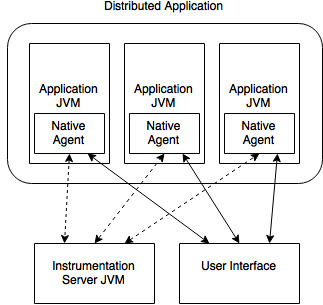
\includegraphics[scale=0.8]{shared_server.png}
 	\caption{Architecture with shared instrumentation server. The dotted lines represent the communication between instrumentation server and the agent, whilst the regular lines represent data collection from the agent to the UI.}
 	\label{fig:shared_server}
 \end{figure}
 
 The other deployment method is that the instrumentation server runs on each application node. This has the advantage of faster communication since  inter-process communication is used to communicate between monitored JVM and the instrumentation server. The disadvantage of this solution is that all classes have to be instrumented on each node since there is no communication between the instrumentation servers. In this solution, the server is started automatically during the native agent initialization. Architecture of this scenario is depicted on the Figure \ref{fig:separated_server}.
 
 \begin{figure}
 	\centering
 	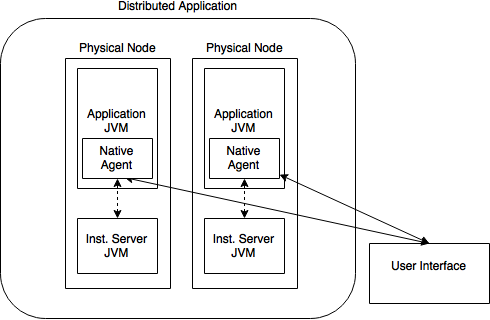
\includegraphics[scale=0.8]{separated_server.png}
 	\caption{Architecture with separated instrumentation server. The dotted lines represent the communication between instrumentation server and the agent, whilst the regular lines represent data collection from the agent to the UI.}
 	\label{fig:separated_server}
 \end{figure}

Except from the cached classes, the server does not contain any application state and it just reacts to the agent requests. It can accept four type of requests:
\begin{itemize}
	\item Request for code instrumentation.
	\item Request for storing bytecode for a class on the server.
	\item Request for sending all helper classes needed by the agent such as the \texttt{Span} class or \texttt{TraceContext} class.
	\item Request to check whether the server contains specific class or not.
\end{itemize}
The server interacts in more ways with the agent, however they are just sub-parts of the communication initiated by one of these 4 request types.	

The instrumentation server needs to deal with several technical problems. The main issue is that the classes which are about to be instrumented require all other dependent classes to be available. The other issue is instrumenting the classes with circular dependencies. The server also performs several optimizations to provide faster response to the agent such as caching the instrumented classes or minimizing the communication when possible. The technical aspects of these issues and the optimizations mentioned above are described in the following sections.
\subsection{Instrumentation}
The instrumentation of the class is triggered by the agent and it's done in two stages. The first stage informs the client whether the class is already on the instrumentation server or not. The second stage is the instrumentation itself. The first stage is initiated by the agent. The server performs the check for class availability in 3 phases:
\begin{enumerate}
	\item Check whether the instrumented bytecode for this class is available.
	\item If not, check whether the original bytecode for this class is available.
	\item If not, check if the class can be loaded using the server's context class loader. This handles the cases where the user builds the instrumentation server together with the application classes or adds the application classes on the instrumentation server classpath for optimization reasons.
\end{enumerate}

The server informs the agent if it does not have the bytecode for the class available and in that case  the agent sends the class to the server. The server registers the received bytecode under the class name. The agent therefore does not have to send the class next time since it's already cached on the instrumentation server.
The second stage follows the first stage immediately. If the server already contains the instrumented class in the cache, the instrumented class is sent right away without instrumenting the class again. If the cache is empty, the class is instrumented and put into the cache.

The code to be  instrumented is specified using the \texttt{MainAgentBuilder} and \texttt{BaseAgentBuilder} classes.
The instrumentation server expects the instance of \texttt{MainAgentBuilder} on the input of its \texttt{start} method. This is an abstract class containing single abstract method \texttt{createAgent(BaseAgentBuilder builder, String pathToHelperClasses)}, where the builder is a wrapper around the Byte Buddy \texttt{AgentBuilder} class, which is used to define the class transformers.

The developer needs to implement this method and specify on which classes and on which methods the instrumentation should happen. Since Byte Buddy is used for writing transformers and interceptors, please read more about Byte Buddy in the Section \ref{sec:byte_buddy}. The server provides several helper methods for creating the transformers and interceptors, which are less verbose then the standard Byte Buddy approaches.

Each transformer has to have associated either an interceptor or advice defining the code to be injected to the original code. Each interceptor implementation has to implement \texttt{Interceptor} interface. This is required for the server to be able to discover all interceptors at run-time without the need for changing the internals of the server. Each implementation of the interceptor needs to register itself in the META-INF directory of the generated JAR in the same way as the span exporters mentioned in the previous section. Custom service loader is then used to locate all classes implementing the \texttt{Interceptor} interface. 

The advices may be used without any special annotations since Byte Buddy in-lines the code defined by the advices into the original code and therefore there is no need to transfer the Advice classes to monitored application.

Even though Byte Buddy takes care about the internals of the instrumentation, the \texttt{BaseAgentBuilder} class is internally properly configured so the instrumentation is defined exactly as desired. The class implements four Byte Buddy listeners used for informing us about the instrumentation progress and allow us to react on the process of the instrumentation. The listeners are:
\begin{itemize}
	\item \texttt{onTransformation} listener is called immediately before the class is instrumented.  Implementation of the listener in the thesis also sends the agent all auxiliary classes required by the instrumented class and the initializers used for setting the static interceptor field on the instrumented class.
	\item \texttt{onIgnored} listener is called when the class is not instrumented. The class is not instrumented when the user does not define any transformer for the specified class.
	\item \texttt{onError} listener is called when some exception occurred during the instrumentation.
	\item \texttt{onComplete} listener is called when instrumentation process completed. It is called after both of \texttt{onTransformation} and \texttt{onIgnored} listeners.
\end{itemize}

Byte buddy requires dependencies for the instrumented class to be available. They are needed because the instrumentation framework needs to know signature of all methods in several cases, for example when the method is overridden in the child class. The dependencies are all the classes specified in the class file such as type of the methods return value or arguments, super class or implemented interfaces. 
By default, Byte Buddy tries to find these dependencies using two classes - \texttt{LocationStrategy} and \texttt{PoolStrategy}. The first class is used to tell Byte Buddy where to look for the raw bytecode of dependent classes. The classes are loaded by context class loader by default, but since the classes are received over the network, custom \texttt{InstrumentorClassloader} class loader is used to handle the class loading. It is a simple class loader which keeps the cache of the classes received from the agent and when a request for instrumentation comes, instead of looking into the class files, it loads the data from the cache in the memory.

However, Byte Buddy internal API does not work with raw bytecode for scanning the further dependencies and obtaining the metadata for the classes. It uses classes \texttt{TypeDescription} and \texttt{PoolStrategy} for this purpose. The first class has a constructor accepting the \texttt{Class} class and created instance contains metadata for the class such as the signature of all methods and fields, list of all interfaces or for example list of constructors. The second class is used for caching the type descriptions so they are not created every time the class is accessed. 

So in overall, class lookup is done in the following two steps:
\begin{enumerate}
	\item Check whether type description for the class is available. If yes, load the type description from the cache.
	\item If the type description is not available, load the class using the \newline \texttt{InstrumentorClassloader}, create type description for the class and put it in the cache.
\end{enumerate}

\subsection{Custom Service Loader}
In order to allow the developer to extend the base instrumentation library service loaders for loading the extensions are used. The service loader is used for two object types: 
\begin{itemize}
	\item \textbf{Custom span exporters} - Each span exporter inherits from the abstract class \texttt{SpanExporter}.
	\item \textbf{Custom Interceptors} - Each interceptor has to implement the interface \texttt{Interceptor}.
\end{itemize} 
The user can create custom span exporter and interceptors by either inheriting the desired class or implementing the required interface and put the name of the class inside the text file in the META-INF directory in the JAR file. The text file has to have the same name as the abstract class or the interface the implementation is for. For example, when user creates a new Interceptor called \texttt{x.y.InterceptorA}, the file \texttt{Interceptor} in the META-INF folder has to contain line \textbf{x.y.InterceptorA}.

Java provides service loader for this purpose. However the standard Java implementation looks up the classes defined as above and automatically creates new instances using the well-known constructors. For the thesis purposes this was unwanted as it is only required to obtain \texttt{Class} object representing the available implementation. Therefore a custom service loader was created for this purpose. This loader works in very similar way as the standard Java one, but instead of returning the instances of loaded services it just returns classes of available services. 

\subsection{JSON Generation}
The data inside spans are internally stored as instances of \texttt{JSONValue} class since in order to support the communication with the default Zipkin UI they need to be exported as JSON. JSON is a lightweight format for exchanging data where the syntax is based on Javascript object notation.

The JSON handling is based on the minimal-json library\footnote{The library is available at \url{https://github.com/ralfstx/minimal-json}.}, however custom simplified implementation was created which fits the theses requirements. Also the number of dependencies is lowered by this decision. 

This JSON support is designed via several classes:
\begin{enumerate}
	\item \textbf{JSONValue}. The abstract ancestor of all JSON types. This type defines common methods to all implementation.
	\item \textbf{JSONString}. Class representing the string type.
	\item \textbf{JSONNumber}. Class representing the numeric types.
	\item \textbf{JSONLiteral}. Class representing the literals \textbf{null}, \textbf{true} and \textbf{false}.
	\item \textbf{JSONArray}. Class representing the JSON arrays. It has support for adding new elements into the array.
	\item \textbf{JSONObject}. Class representing the JSON objects. It has support for adding a new items in the object.
\end{enumerate}

Each \textbf{JSONValue} can be printed as valid JSON string where the printing is driven by\texttt{JSONStringBuilder} class. This class is also responsible for escaping the characters according to JSON standards. The default printer prints the data without any formatting as one line, however \texttt{JSONPrettyStringBuilder} prints the data in more human-readable format. The second printer is usually used for debugging purposes and the first one for real usage as the size of the data is smaller in this case.

\section{User Interface}
\label{sec:zipkin_ui}.
The user interface receives spans and presents them in a hierarchical way so the relationships between different nodes can be seen easily. The important feature of the user interface is that the data for a single span can be sent incrementally. This means that several JSONs representing the same span can be sent with different annotations and the user interface merges these spans into single one and presents all annotations under the given span. This allow the tool to send part of data from the sender side and part of data from the receiver side directly to the user interface instead of sending the data back on forth to send them as one single complete span.

The thesis is using Zipkin as default user interface. The default data format for exporting spans is designed in order to be understandable by this user interface. The user is however still able to change the data format to support custom user interface via custom span exporter class. This section gives an overview of Zipkin user interface and describes the Zipkin data model


\begin{figure}
	\centering
	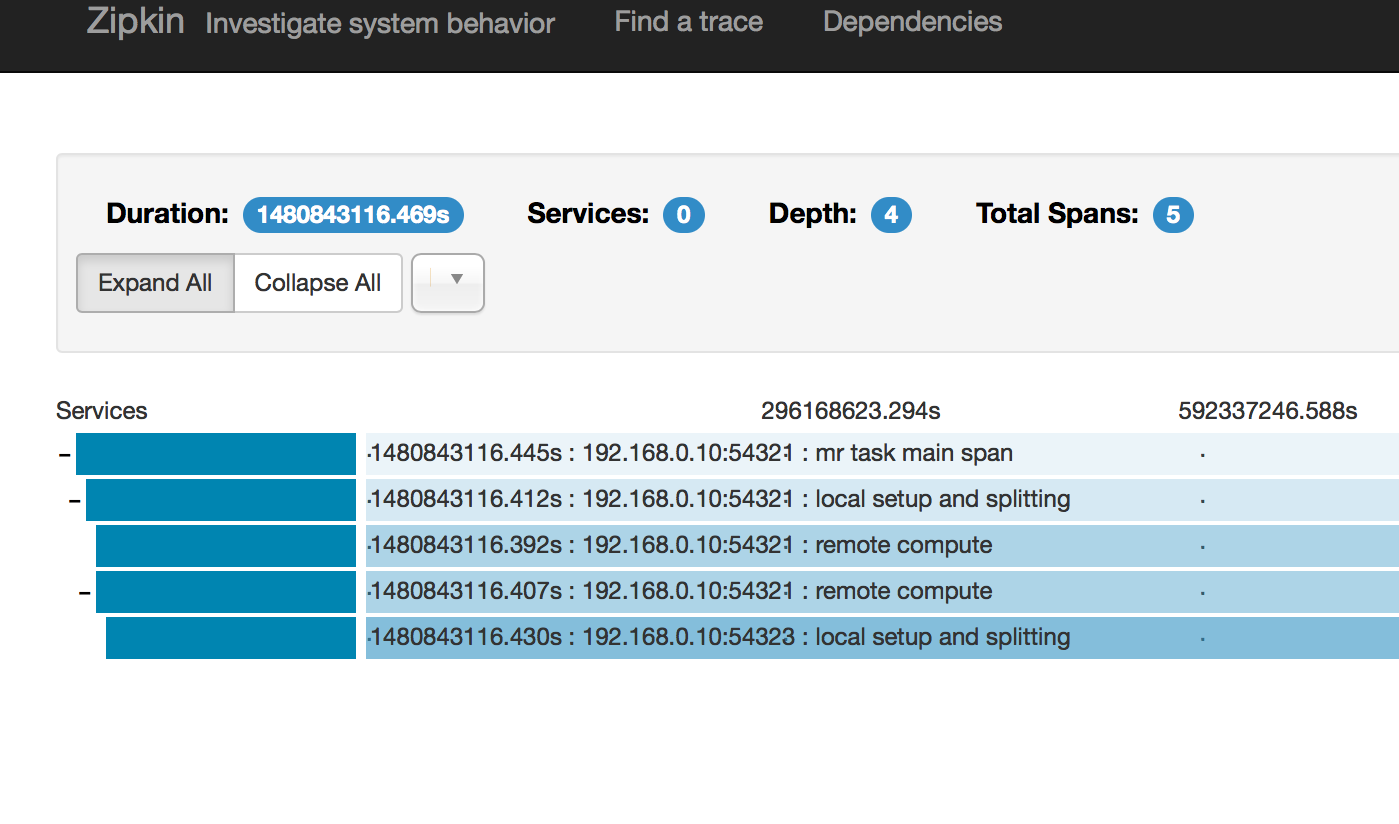
\includegraphics[scale=0.5]{zipkin_ui_example.png}
	\caption{Example of Zipkin UI}
	\label{fig:zipkin_ui}
\end{figure}

Each span in the UI is clickable and all the additional information can bee seen at that level. In this thesis the stack trace are also collected at each span for monitoring purposes. Example of such information screen can be seen on the Figure \ref{fig:zipkin_ui_detail}.
\begin{figure}
	\centering
	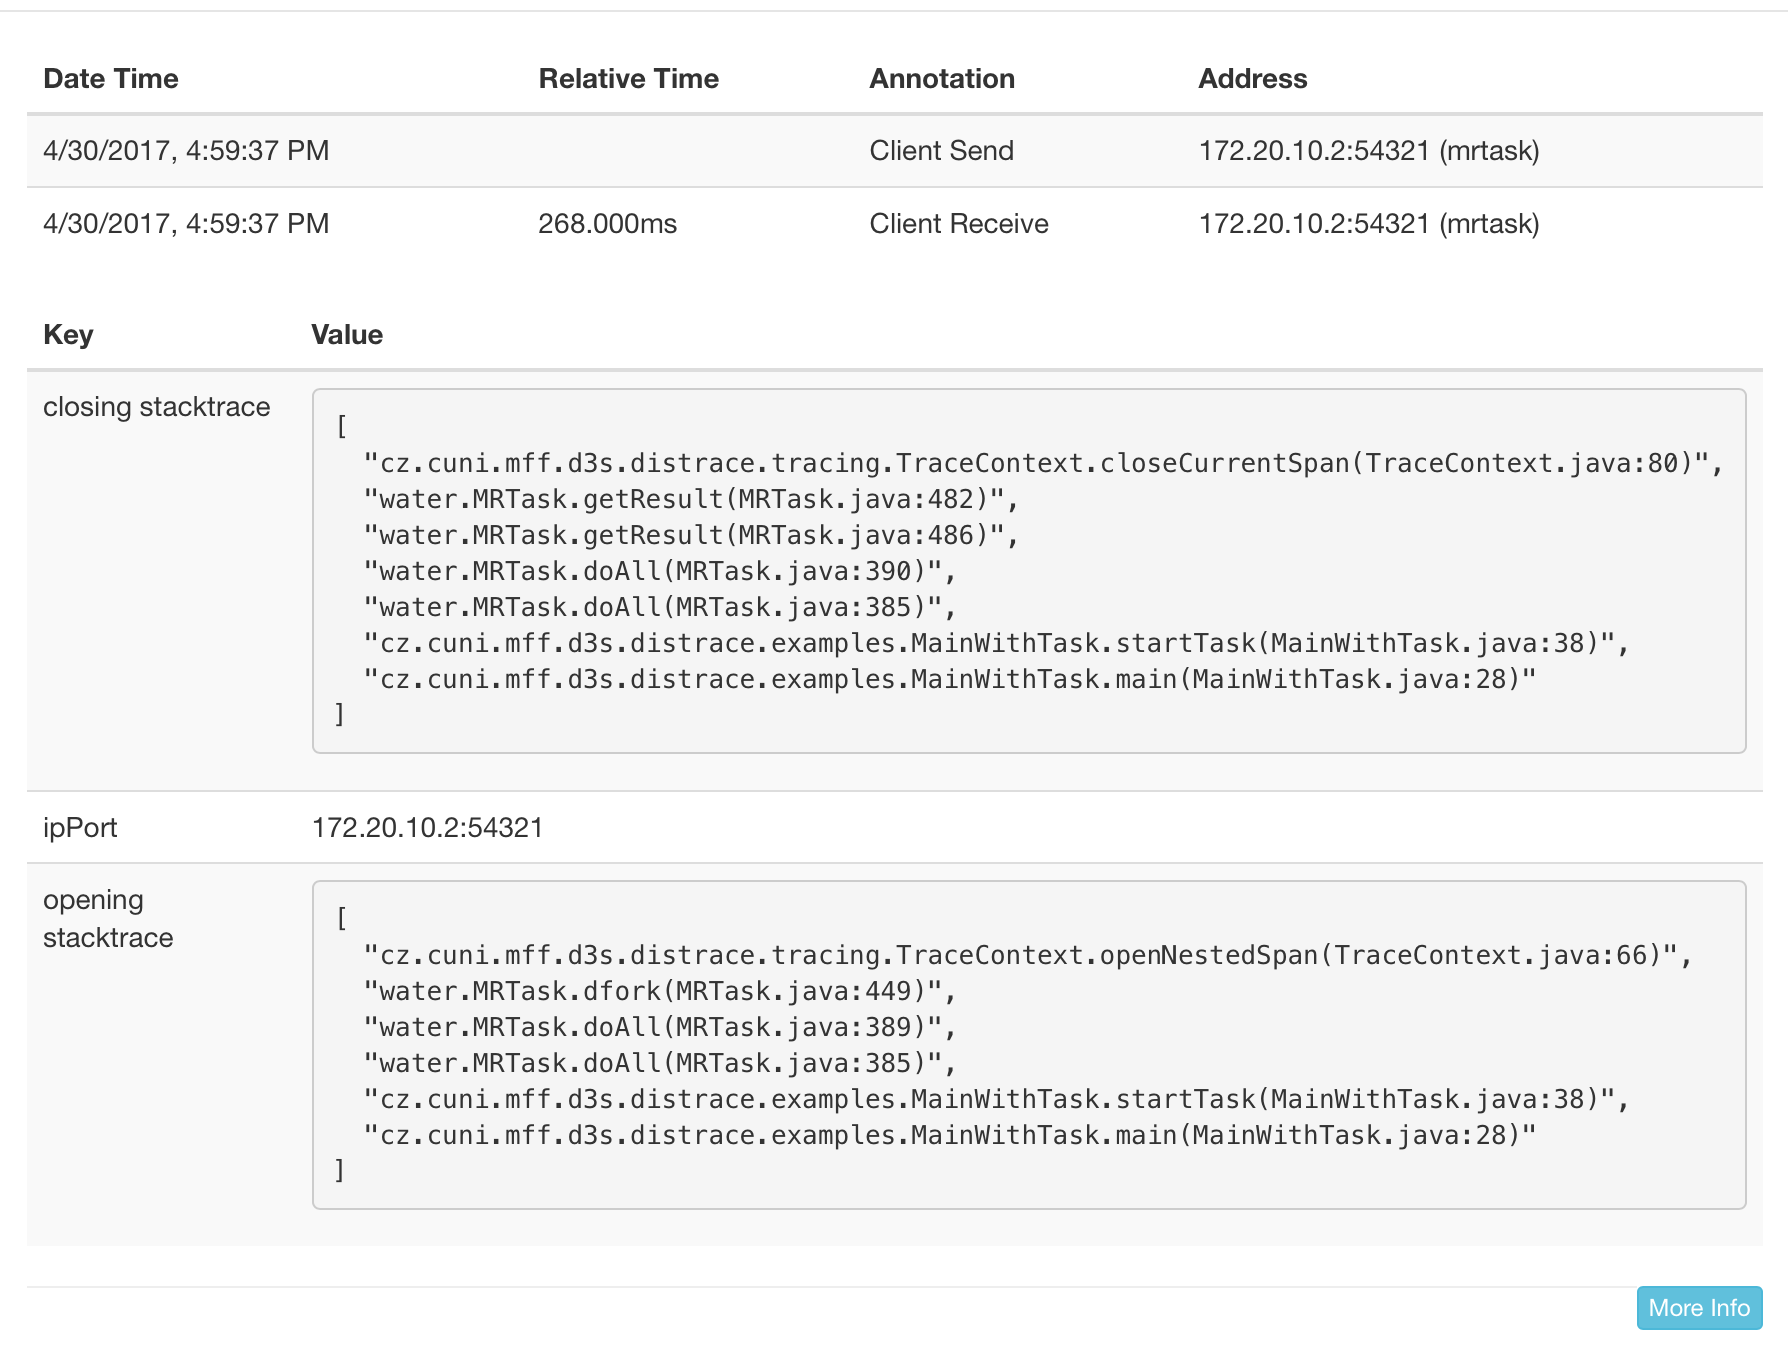
\includegraphics[scale=0.4]{zipkin_ui_detail.png}
	\caption{Example of the detail span information.}
	\label{fig:zipkin_ui_detail}
\end{figure}
\subsection{Zipkin Data Model}
Zipkin requires data to be sent in JSON format. Requests to UI are sent as JSON arrays where the array elements are the spans. Zipkin understands the following fields of Span object:
\begin{itemize}
	\item \textbf{traceId} - unique id representing the complete trace. It can be either 128 or 64 bit long.
	\item \textbf{name} - human readable span name
	\item \textbf{id} - id of this span. At the current implementation, Zipkin UI supports span ids only to be 64-bit long.
	\item \textbf{parentId} - parent id of the current span.
	\item \textbf{timestamp} - the time when the span was created.
	\item \textbf{duration} - the duration of the span. It is the duration between the span creation and span closing.
	\item \textbf{annotations} - array containing standard Zipkin annotations. These annotations can be handled by user interface in specific way since the user interface understands the meaning of the content. The documentation specifies the following annotations:
	\begin{itemize}
		\item \textbf{cr} : timestamp of client receiving the span
		\item \textbf{cs} : timestamp of client sending the span
		\item \textbf{sr} : timestamp of server receiving the span
		\item \textbf{ss} : timestamp of server receiving the span
		\item \textbf{ca} : client address
		\item \textbf{sa} : server address
	\end{itemize}
	\item \textbf{binaryAnnotations} - array of custom annotations. For example collected stack traces are sent as a binary annotation.
\end{itemize}

Except the \textit{annotations} and \textit{binaryAnnotations} fields, the fields are of simple string or number type. Annotations are objects with the three fields - annotation value, annotation name and the endpoint. Endpoint is another object specifying the address and port at the code where the span or particular annotation was recorded. Endpoints can also specify service name which may be used to search for particular spans.

Full example of data sent to Zipkin can be:
\begin{lstlisting}[emph={traceId, name, id, timestamp, duration, annotations, value, endpoint, serviceName, ipv4, port, binnaryAnnotations, key},emphstyle={\textbf}]
[
 {
    "traceId": "123456789abcdef",
    "name": "query",
    "id": "abcd1",
    "timestamp": 1458702548467000,
    "duration": 100743,
    "annotations": [
      {
        "timestamp": 1458702548467000,
        "value": "sr"
        "endpoint": {
          "serviceName": "example",
          "ipv4": "192.168.1.2",
          "port": 9411
        },
      }
    ],
    "binaryAnnotations": [
      {
        "key": "bytes_sent",
        "value": "1783"
        "endpoint": {
          "serviceName": "example",
          "ipv4": "192.168.1.2",
          "port": 9411
        },
      }
    ]
 }
]
\end{lstlisting}


